\ifx\wholebook\relax\else
\documentclass{report}
\usepackage{times}
\usepackage{epsfig}
\usepackage{alltt}
\usepackage{xspace}
\usepackage{graphicx}
\usepackage{ifpdf}
\usepackage{ifthen}
\usepackage{amsmath}
\usepackage{a4wide}

\graphicspath{{figures/}} 

\ifpdf
\DeclareGraphicsExtensions{.pdf, .jpg, .tif, .png}
\else
\DeclareGraphicsExtensions{.eps, .jpg}
\fi

\newboolean{toseecomment}
\setboolean{toseecomment}{false}
%%change to false to hidde comment 
\newcommand{\comment}[1]{\ifthenelse{\boolean{toseecomment}}{$\blacktriangleright$ \textit{#1}$\blacktriangleleft$}{}}

\newcommand{\commented}[1]{}

\newboolean{seevwspecific}
\setboolean{seevwspecific}{true}
\newcommand{\vwspecific}[1]{\ifthenelse{\boolean{seevwspecific}}{#1}{}}

\newboolean{seecategoryspecific}
\setboolean{seecategoryspecific}{false}
\newcommand{\categoryspecific}[1]{\ifthenelse{\boolean{seecategoryspecific}}{#1}{}}

\newboolean{seestorespecific}
\setboolean{seestorespecific}{true}
\newcommand{\storespecific}[1]{\ifthenelse{\boolean{seestorespecific}}{#1}{}}

\newboolean{seesqueakspecific}
\setboolean{seesqueakspecific}{false}
\newcommand{\squeakspecific}[1]{\ifthenelse{\boolean{seesqueakspecific}}{#1}{}}


\newcommand{\category}[0]
{\ifthenelse{\boolean{seestorespecific}}
	{package\xspace}
	{category\xspace}}

\newcommand{\ct}[1]{\texttt{#1}\xspace}
\newcommand{\stc}[1]{{\small {\sf #1}}\xspace}
\newcommand{\ST}{{\textsc Smalltalk}\xspace}
\newcommand{\tab}{\makebox[4em]{}}
\newcommand{\ttt}[1]{{\tt #1}}
\newcommand{\chev}{\ttt{>>}}
\newcommand{\vw}{VisualWorks\xspace}
\newcommand{\sq}{Squeak\xspace}
\newcommand{\store}{Store\xspace}
\renewcommand{\chaptername}{Exercise}
\newcommand{\exercise}{\vspace{0.2cm}\noindent \textbf{Exercise:}\xspace}

\newsavebox{\fminibox}
\newlength{\fminilength}

% Fait un truc encadre
\newenvironment{fminipage}[1][\linewidth]
  {\setlength{\fminilength}{#1-2\fboxsep-2\fboxrule}
        \begin{lrbox}{\fminibox}\begin{minipage}{\fminilength}}
  { \end{minipage}\end{lrbox}\noindent\fbox{\usebox{\fminibox}}}

% Pareil mais pas encadre (a utiliser pour ne pas couper une fonction

\newenvironment{nminipage}[1][\linewidth]
  {\setlength{\fminilength}{#1}
        \begin{lrbox}{\fminibox}\begin{minipage}{\fminilength}}
  { \end{minipage}\end{lrbox}\noindent\mbox{\usebox{\fminibox}}}

% Un alltt encadre
\newenvironment{falltt}
  {\vspace*{0.3cm}\begin{fminipage}\begin{alltt}}
  {\end{alltt}\end{fminipage}\vspace*{0.3cm}}

% Un alltt pas encadre
\newenvironment{nalltt}
  {\vspace*{0.3cm}\begin{nminipage}\begin{alltt}}
  {\end{alltt}\end{nminipage}\vspace*{0.3cm}}

% Une fonction encadree
\newenvironment{ffonction}[1]
  {\begin{fonction}[#1]
        \begin{fminipage}
\begin{alltt}
\rule{\linewidth}{0.5pt}}
{\end{alltt}\end{fminipage}\end{fonction}}

\newenvironment{codeonepage}
  {\begin{nminipage}\vspace*{0.2cm}\hrule\vspace*{0.1cm}
\begin{alltt}}
  {\end{alltt} \vspace*{-0.2cm}\hrule \vspace*{0.2cm} \end{nminipage}}

\newenvironment{code}
  {\vspace*{0.1cm}\hrule\vspace*{-0.1cm}\begin{alltt}}
  {\end{alltt}\vspace*{-0.2cm}\hrule \vspace*{0.1cm}}



\begin{document}
\fi

\chapter{Counter Example}
This document provides the initial exercise you should do to be
familiar with Smalltalk syntax and VisualWorks 7.


\section*{A Simple Counter}
We want you to implement a simple counter that follows the small example given
below. Please note that we will ask you to define a test for this example.

\begin{code}
|counter|
counter := SimpleCounter new.
counter increment; increment.
counter decrement.
counter value = 1
\end{code}


\section*{Creating your own class}
In this part you will create the first class. In traditional Smalltalk environments a class is associated with a category (a folder containing the classes of your project). 

\storespecific{When we are using \store, categories are replaced by package. 
Therefore in \vw with \store you define a package and define your class within this package.}
The steps we will do are the same ones every  time you create a class, so memorize them well. We are going to create a class \texttt{SimpleCounter} in a \category called \texttt{DemoCounter}. Note that are you will be all versioning your code in the \store database your package have to have a different name. So prefix them with your initials.

\storespecific{
\subsection*{Creating a Package}
In the System Browser, click on \texttt{Local Image} (left button
of the mouse) and select \texttt{New}$>>$\texttt{Package}. The
system will ask you a name. You should write \texttt{DemoCounter}.
This new package will be created and added to the list.}

\squeakspecific{
\subsection*{Creating a Class category}
In the System Browser, click on the left pane and select add. The
system will ask you a name. You should write \texttt{DemoCounter}.
This new \category will be created and added to the list.}

\vwspecific{\subsection*{With Namespace}
In \vw you can also define your own namespace. If you do so you will have to define your namespace then define the class in this namespace. For now we suggest you to use the default namespace called \ct{Smalltalk}.}

\subsection*{Creating a Class}


\storespecific{
\begin{figure}[htbp]
\begin{center}
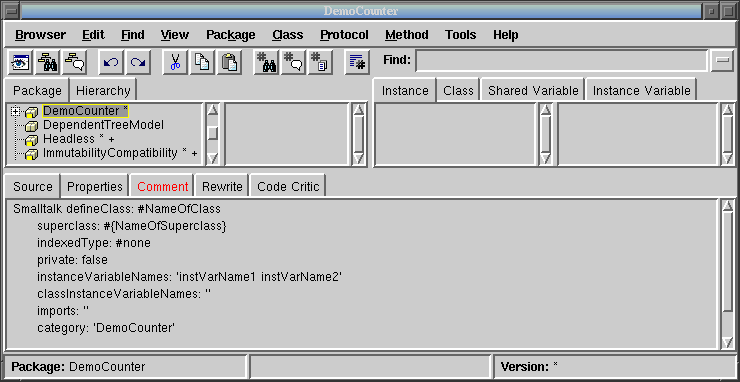
\includegraphics[scale=0.5]{nlesson3Fig4Package}
\caption{Your package is created.}
\end{center}
\end{figure}}

\categoryspecific{
\begin{figure}[htbp]
\begin{center}
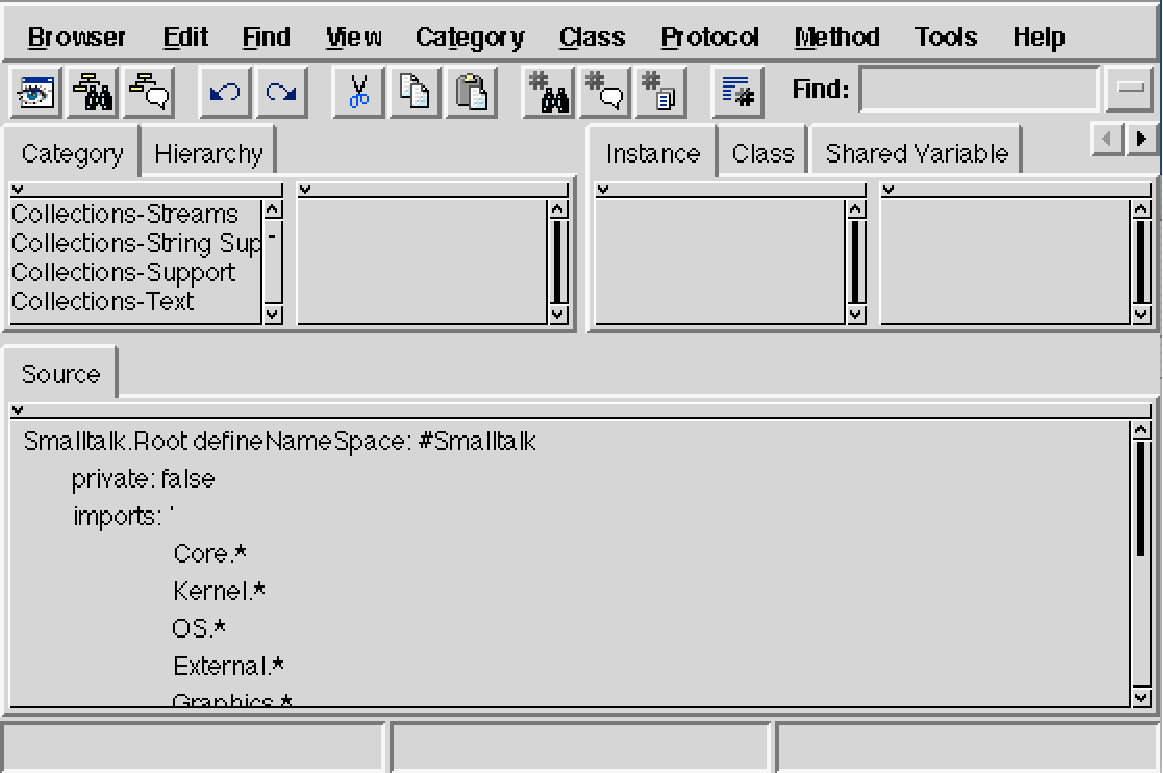
\includegraphics[scale=0.5]{nlesson3Fig4CategoryVW}
\caption{Your category is created.}
\end{center}
\end{figure}}

Creating a class requires five steps. They consist basically of
editing the class definition template to specify the class you
want to create. \storespecific{\textit{Before you begin, make sure that only the package \texttt{DemoCounter} is selected.}}

\begin{enumerate}
\item \textbf{Superclass Specification}. First, you should replace
the word \texttt{NameOfSuperclass} with the word \texttt{\vwspecific{Core.}Object}\vwspecific{\footnote{We will see when we will be building a user interface for this object that we will change its superclass}}. Thus, you specify the superclass of the class you are
creating. 

\item \textbf{Class Name}. Next, you should fill in the name of
your class by replacing the word \texttt{NameOfClass} with the
word \texttt{SimpleCounter}. Take care that the name of the class
starts with a capital letter and that you do not remove the \#
sign in front of \texttt{NameOfClass}.

\item \textbf{Instance Variable Specification}. Then, you should
fill in the names of the instance variables of this class. We need
one instance variable called \texttt{value}. You add it by
replacing the words \textit{instVarName1} and
\textit{instVarName2} with the word \texttt{value}.Take
care that you leave the string quotes!

\item \textbf{Class Variable Specification}. As we do not need any class variable make sure that the argument  for the class instance variables is an empty string (\ct{classInstanceVariableNames: ''}). 

\item \textbf{Compilation}. That's it! We now have a filled-in
class definition for the class \ct{SimpleCounter}. To define it, we still have to \textbf{compile} it. Therefore,
select the \textbf{accept} option from the operate menu
(right-click button of the mouse). The class
\texttt{SimpleCounter} is now compiled and added to the system.
\end{enumerate}

As we are disciplined developers, we provide a comment to
\texttt{SimpleCounter} class by clicking \textbf{Comment} tab of
the class definition. You can write the following comment:

\begin{code}
SimpleCounter is a concrete class which supports incrementing
and decrementing a counter.

Instance Variables:\\
value\tab \texttt{<}Integer\texttt{>}
\end{code}

Select \textbf{accept} to store this class comment in the class.


\section*{Defining protocols and methods}
This part show how to use the System Browser to add protocols
and methods. 


\subsection*{Creating and Testing methods}
The class we have defined has one instance variable \ct{value}. You should
remember that in Smalltalk, everything is an object, that instance variables are private to the object and  that the only way to interact with an object is by sending messages to them.

Therefore, there is no other mechanism to access the instance variables
from outside an object than sending a message to the object. What you can do is define messages that return the value of the instance variable of a class. Such methods are called \textbf{accessors}, and it is a common practice to always define and use them. We start to create an accessor method for our
instance variable \texttt{value}.

Remember that every method belongs to a protocol. These protocols are just
a group of methods without any language semantics, but convey important
navigation information for the reader of your class. Although protocols
can have any name, Smalltalk programmers follow certain conventions for
naming these protocols. If you define a method and are not sure what
protocol it should be in, first go through existing code and try to
find a fitting name.


\paragraph{An important remark:} Accessors can be defined in protocols
\ct{accessing} or \ct{private}.  Use the
\ct{accessing} protocol when a client object (like an
interface) really needs to access your data. Use \ct{private}
to clearly state that no client should use the accessor. This is
purely a convention. There is no way in Smalltalk to enforce
access rights like private in C++ or Java.  To emphasize that objects are
not just data structure but provide services that are more
elaborated than just accessing data, put your accessors  in a
\ct{private} protocol. As a good practice, if you are not sure
firstly define your accessors in a \ct{private} protocol and
once some clients really need access to some specific data, create
a new protocol \ct{accessing} and move your methods there. Note
that this discussion does not seem to be very important in the
context of this specific simple example. However, this question is
central to the notion of object and encapsulation of the data. An
important side effect of this discussion is that you should always
ask yourself when you, as a client of an object, are using an
accessor if the object is really well defined and if it does not
need extra functionality.

\exercise  Decide in which protocol you are going to put the
accessor for value. We now create the accessor method for
the instance variable \ct{value}. Start by selecting
the class \ct{DemoCounter} in a browser, and make sure the
\texttt{Instance} tab is selected. Create a new protocol
clicking the right-button of the mouse and choosing \ct{New},
and give a name. Select the newly created protocol. Then in the bottom pane, the edit field displays a method template laying out the default structure
of a method. Replace the template with the following method
definition.

\begin{code}
value
  "return the current value of the value instance variable"

  ^value
  
\end{code}

This defines a method called \ct{value}, taking no
arguments, having a method comment and returning the instance
variable \ct{value}. Then choose \textbf{accept} in the
operate menu (left button of the mouse) to compile the method. You
can now test your new method by typing and evaluating the next
expression in a Workspace, in the Transcript, or any text editor \ct{SimpleCounter new value}.

\vwspecific{A workspace can be showed up by clicking on the last icon of the launcher as shown in Figure~\ref{fig:launcher}.}

\vwspecific{
\begin{figure}[htbp]
\begin{center}
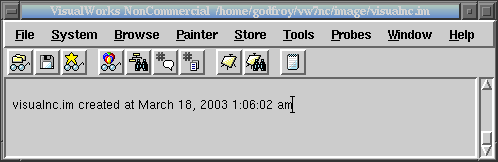
\includegraphics[scale=0.5]{nlesson1Fig1.png}
\caption{The Launcher of VisualWorks.\label{fig:launcher}}
\end{center}
\end{figure}}


This expression first creates a new instance of
\ct{SimpleCounter}, and then sends the message
\ct{value} to it and retrieve the current value of
\ct{value}. This should return nil (the default value
for noninitialised instance variables; afterwards we will create
instances where \ct{value} has a reasonable default
initialisation value). 


\exercise  Another method that is normally used besides the
accessor method is a so-called mutator method. Such a
method is used to change the value of an instance variable from a
client. For example, the next expression first create a new
\ct{SimpleCounter} instance and then sets the value of
\ct{value} to 7: \ct{SimpleCounter new value: 7}


This mutator method does not currently exist, so as an exercise
write the method \ct{value:} such that, when invoked on
an instance of \ct{SimpleCouter}, the \ct{value}
instance variable is set to the argument given to the message.
Test your method by typing and evaluating the expression above.

\exercise Implement the following methods in the protocol operations.

\begin{verbatim}
increment
    self value: self value + 1
decrement
    self value: self value - 1
\end{verbatim}

\exercise Implement the following methods in the protocol printing
\begin{verbatim}
printOn: aStream
    super printOn: aStream.
    aStream nextPutAll: ' with value: ', 
    							self  value printString.
    aStream cr.
\end{verbatim}

Now test the methods \ct{increment} and \ct{decrement} but pay attention that the counter value is not initialized. Try \ct{SimpleCounter new value: 0; increment ; value}.
Note that the method \ct{printOn:} is used when you print an
object or click on \ct{self} in an inspector. 

\subsection*{Adding an instance creation method}
When we create a new instance of the class \ct{SimpleCounter}
using the message \ct{new}, we would like to obtain a well
initialized instance. To do so, we need to override the method
\ct{new} to add a call to an initialization method (invoking
an \ct{initialize} method is a very common practice! Ask for
the senders of \ct{initialize}). Notice that \ct{new} is always
sent to a class. This means we have to define the new method on
the class side. To define an instance creation method like the
method \ct{new} you should be on the class side, so you click
on the \ct{Class} tab. 

\exercise Define a new protocol called \ct{instance creation},
and implement the method \ct{new} as follows:

\begin{code}
new
   "Create and return an initialized instance of SimpleCounter"
   |newInstance|
   newInstance := super new.
   newInstance initialize.
   ^ newInstance
\end{code}

This code returns a new and well initialized instance. We first
create a new instance by calling the normal creation method
(\ct{super new}), then we assign this new created instance
into the temporary variable called \ct{newInstance}. Then we
invoke the \ct{initialize} method on this new created instance
via the temporary variable and finally we return it.

Note that the previous method body is strictly equivalent to
the following one. Try to understand why they are equivalent.

\begin{code}
new
   "Create and return an initialized instance of SimpleCounter"

   ^ super new initialize
\end{code}

\subsection*{Adding an instance initialization method}
Now we have to write an initialization method that sets a default
value to the \ct{value} instance variable. However, as
we mentioned the \ct{initialize} message is sent to the newly
created instance. This means that the \ct{initialize} method
should be defined at the instance side as any method that is sent
to an instance of \ct{SimpleCounter} like \ct{increment}
and \ct{decrement}. The \ct{initialize} method does not
have specific and predefined semantics; it is just a convention to
name the method that is responsible to set up the instance
variable default values.

Therefore at the instance side, you should create a protocol
\texttt{initialize-release}, and create following method (the body
of this method is left blank. Fill it in!).

\begin{code}
initialize
   "set the initial value of the value to 0"
\end{code}

\paragraph{Remark.} As we already mentioned, the \ct{initialize} 
method is not automatically invoked by the method \ct{new}.
We had to override the method \ct{new} to call the
\ct{initialize} method. This is a weakness of the Smalltalk
libraries, so you should always check if the class that you are
creating inherits from a \ct{new} method that implements the
call to the \ct{initialize} method. It is a good practice to
add such a calling structure (\ct{new} calling
\ct{initialize}) in the root of the your class hierarchy. This
way you share the calling structure and are sure that the
\ct{initialize} method is always called for all your classes.

Now create a new instance of class \ct{SimpleCounter}. Is it
initialized by default? The following code should now work without
problem: \ct{SimpleCounter new increment}

\subsection*{Another instance creation method}
If you want to be sure that you have really understood the
distinction between instance and class methods, you should define
now a different instance creation method named
\ct{withValue:}. This method receives an integer as argument
and returns an instance of \ct{SimpleCounter} with the
specified value. The following expression should return 20.
\ct{(SimpleCounter withValue: 19) increment ; value}


\paragraph{A Difficult Point}
Let us just think a bit! To create a new instance we said that we
should send messages (like \ct{new} and \ct{basicNew}) to
a class. For example to create an instance of
\ct{SimpleCounter} we sent \ct{new} to
\ct{SimpleCounter}. As the classes are also objects in
Smalltalk, they are instances of other classes that define the
structure and the behavior of classes. One of the classes that
represents classes as objects is \ct{Behavior}. Browse the
class \ct{Behavior}. In particular, \ct{Behavior} defines
the methods \ct{new} and \ct{basicNew} that are
responsible of creating new instances. If you did not redefine the
new message locally to the class of \ct{SimpleCounter}, when
you send the message \ct{new} to the class
\texttt{SimpleCounter}, the new method executed is the one defined
in \ct{Behavior}.

\section*{SUnit}
Download the tutorial SUnit Explained from http://www.iam.unibe.ch/$\sim$ducasse/\-WebPages\-/Books.html and define a TestCase with several tests for the SimpleCounter class. To open the test runner execute \ct{TestRunner open}.

\section*{Saving your Work}
\storespecific{To save our work, simply publish your package. Saving the image is also one way to save your work but publishing it save the code in the database.}


\ifx\wholebook\relax\else\end{document}\fi
